\documentclass[a4paper,10pt]{article}
\usepackage{amsmath}
\usepackage{amsthm}
\newtheorem{mydef}{Definition}
\usepackage{url, hyperref}
\usepackage{amsthm}
\usepackage{amsfonts}
\usepackage{amssymb}
\newtheorem{theorem}{Theorem}
\newtheorem{lemma}{Lemma}
\usepackage{fullpage}
\usepackage{tikz}
\usepackage{float}
\usepackage{listings}
\usepackage{color}
\usepackage{mathtools}
\usepackage[T1]{fontenc}
\usepackage{subfigure}
\usepackage{algorithm}
\usepackage{algpseudocode}
\bibliographystyle{plain}

\begin{document}
\begin{titlepage}
\begin{center}
\textsc{\LARGE Stellenbosch University}\\[1.5cm]

\textsc{\Large Applied Mathematics Honours Project}\\[0.5cm]

{ \huge \bfseries Efficient segmentation algorithms for shark fin
identification \\[0.4cm] }

\begin{minipage}{0.4\textwidth}
\begin{center} \large
\emph{Author:}\\
L. Cilli\'{e}, 16010450
\end{center}
\end{minipage}
\begin{minipage}{0.4\textwidth}
\begin{center} \large
\emph{Project Advisors:} \\
Prof. B.M. Herbst and Dr. S.J van der Walt
\end{center}
\end{minipage}

\vfill

\vspace{20mm}

18 October 2013
\end{center}

\end{titlepage}

\newpage
\tableofcontents

\newpage
\section{Problem statement and motivation}
\subsection{}
Just as humans are identified by their fingerprints, sharks have an unique
dorsal fin structure.  Identifying shark sightings these days can be very
valuable.  In order to do that and also to match shark sightings, photos of
shark fins, as will be shown in the proposal, will be analysed by a computer. 
This will consist of comparing the edges in the image and segmenting the
foreground, the shark fin being most prominent,  from the background, the sea. 
Although the photos provided are of a good quality and only include the fin, the
foreground and background properties can still vary significantly, making this a
non-trivial problem.  This project aims to investigate efficient segmentation
algorithms for shark fin identification.  The approach will consist of
evaluating (by means of a computer) different methods for classifying foreground
and background, as well as segmenting the foreground successfully.  By doing so,
the burden on biological researchers can be reduced.  \\

The idea behind the project originated when PhD
student in Marine Biology, Ms. Sara Andreotti, approached Dr. van der Walt for
help regarding a problem she encountered in her research.
The problem presented was
as follows.  The work Ms. Andreotti does involve going out into the ocean,
taking photographs of shark fins and identifying those sharks to later study their ecological and behavioural
patterns, for example.
All these photos are put into a databases. But to
make any reliable conclusions, such as: Have we seen this shark before?  How
many
times? Where? When?, there has to be some form of identification in the
databases. 
The goal is to group photos of a certain individal together.  We
already know that it is possible to categorize each image, because of the
uniqueness of the dorsal fin.  One would just have to find a way to match new
input data with existing images in the databases.  One can only imagine the
diffuculty in doing this manually. 
Since Ms. Andreotti's
focus is on the distribution and movements of sharks and not on developing new
software, we can make a substantial contribution by researching this topic. 

Below are a few examples of the data used in this research project.

\begin{figure}[H]
\centering
\mbox{\subfigure[]{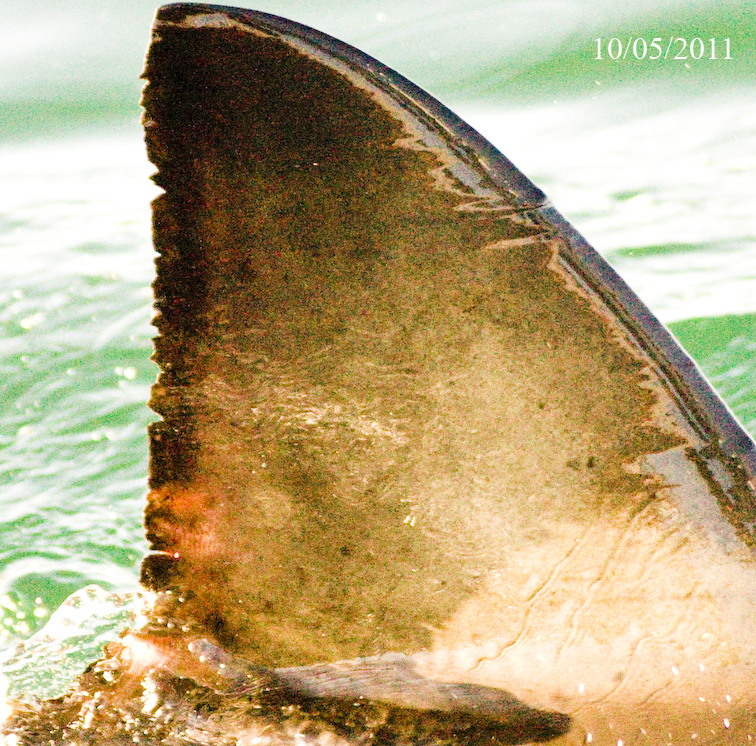
\includegraphics[width=2in]{haai1.jpg}} \quad
\subfigure[]{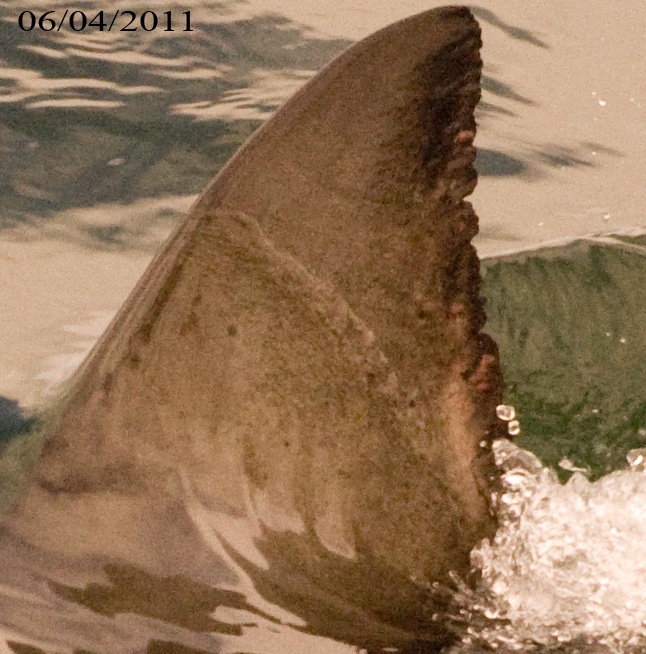
\includegraphics[width=2in]{haai4.jpg}} \quad
\subfigure[]{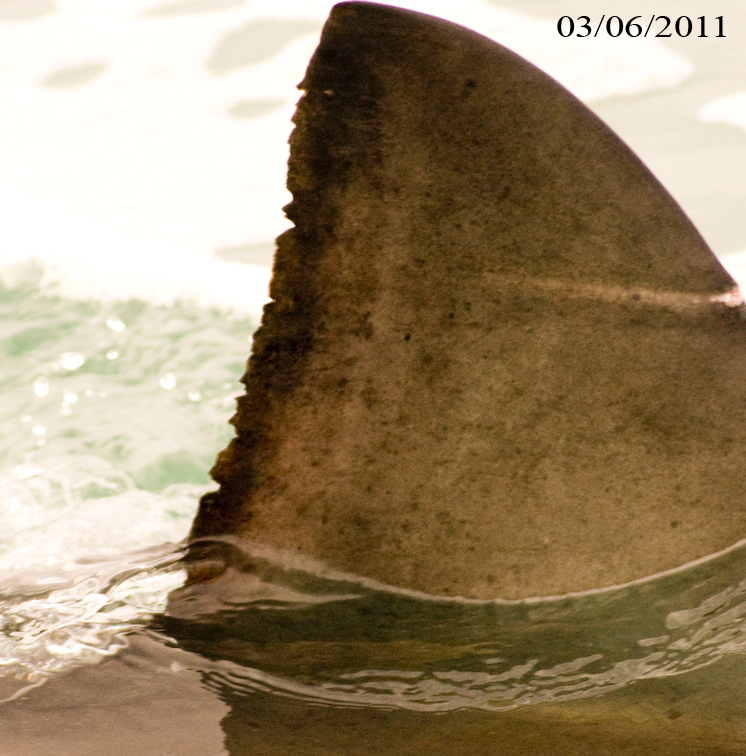
\includegraphics[width=2in]{haai2.jpg}}}
\end{figure}

\begin{figure}[H]
\centering
\mbox{\subfigure[]{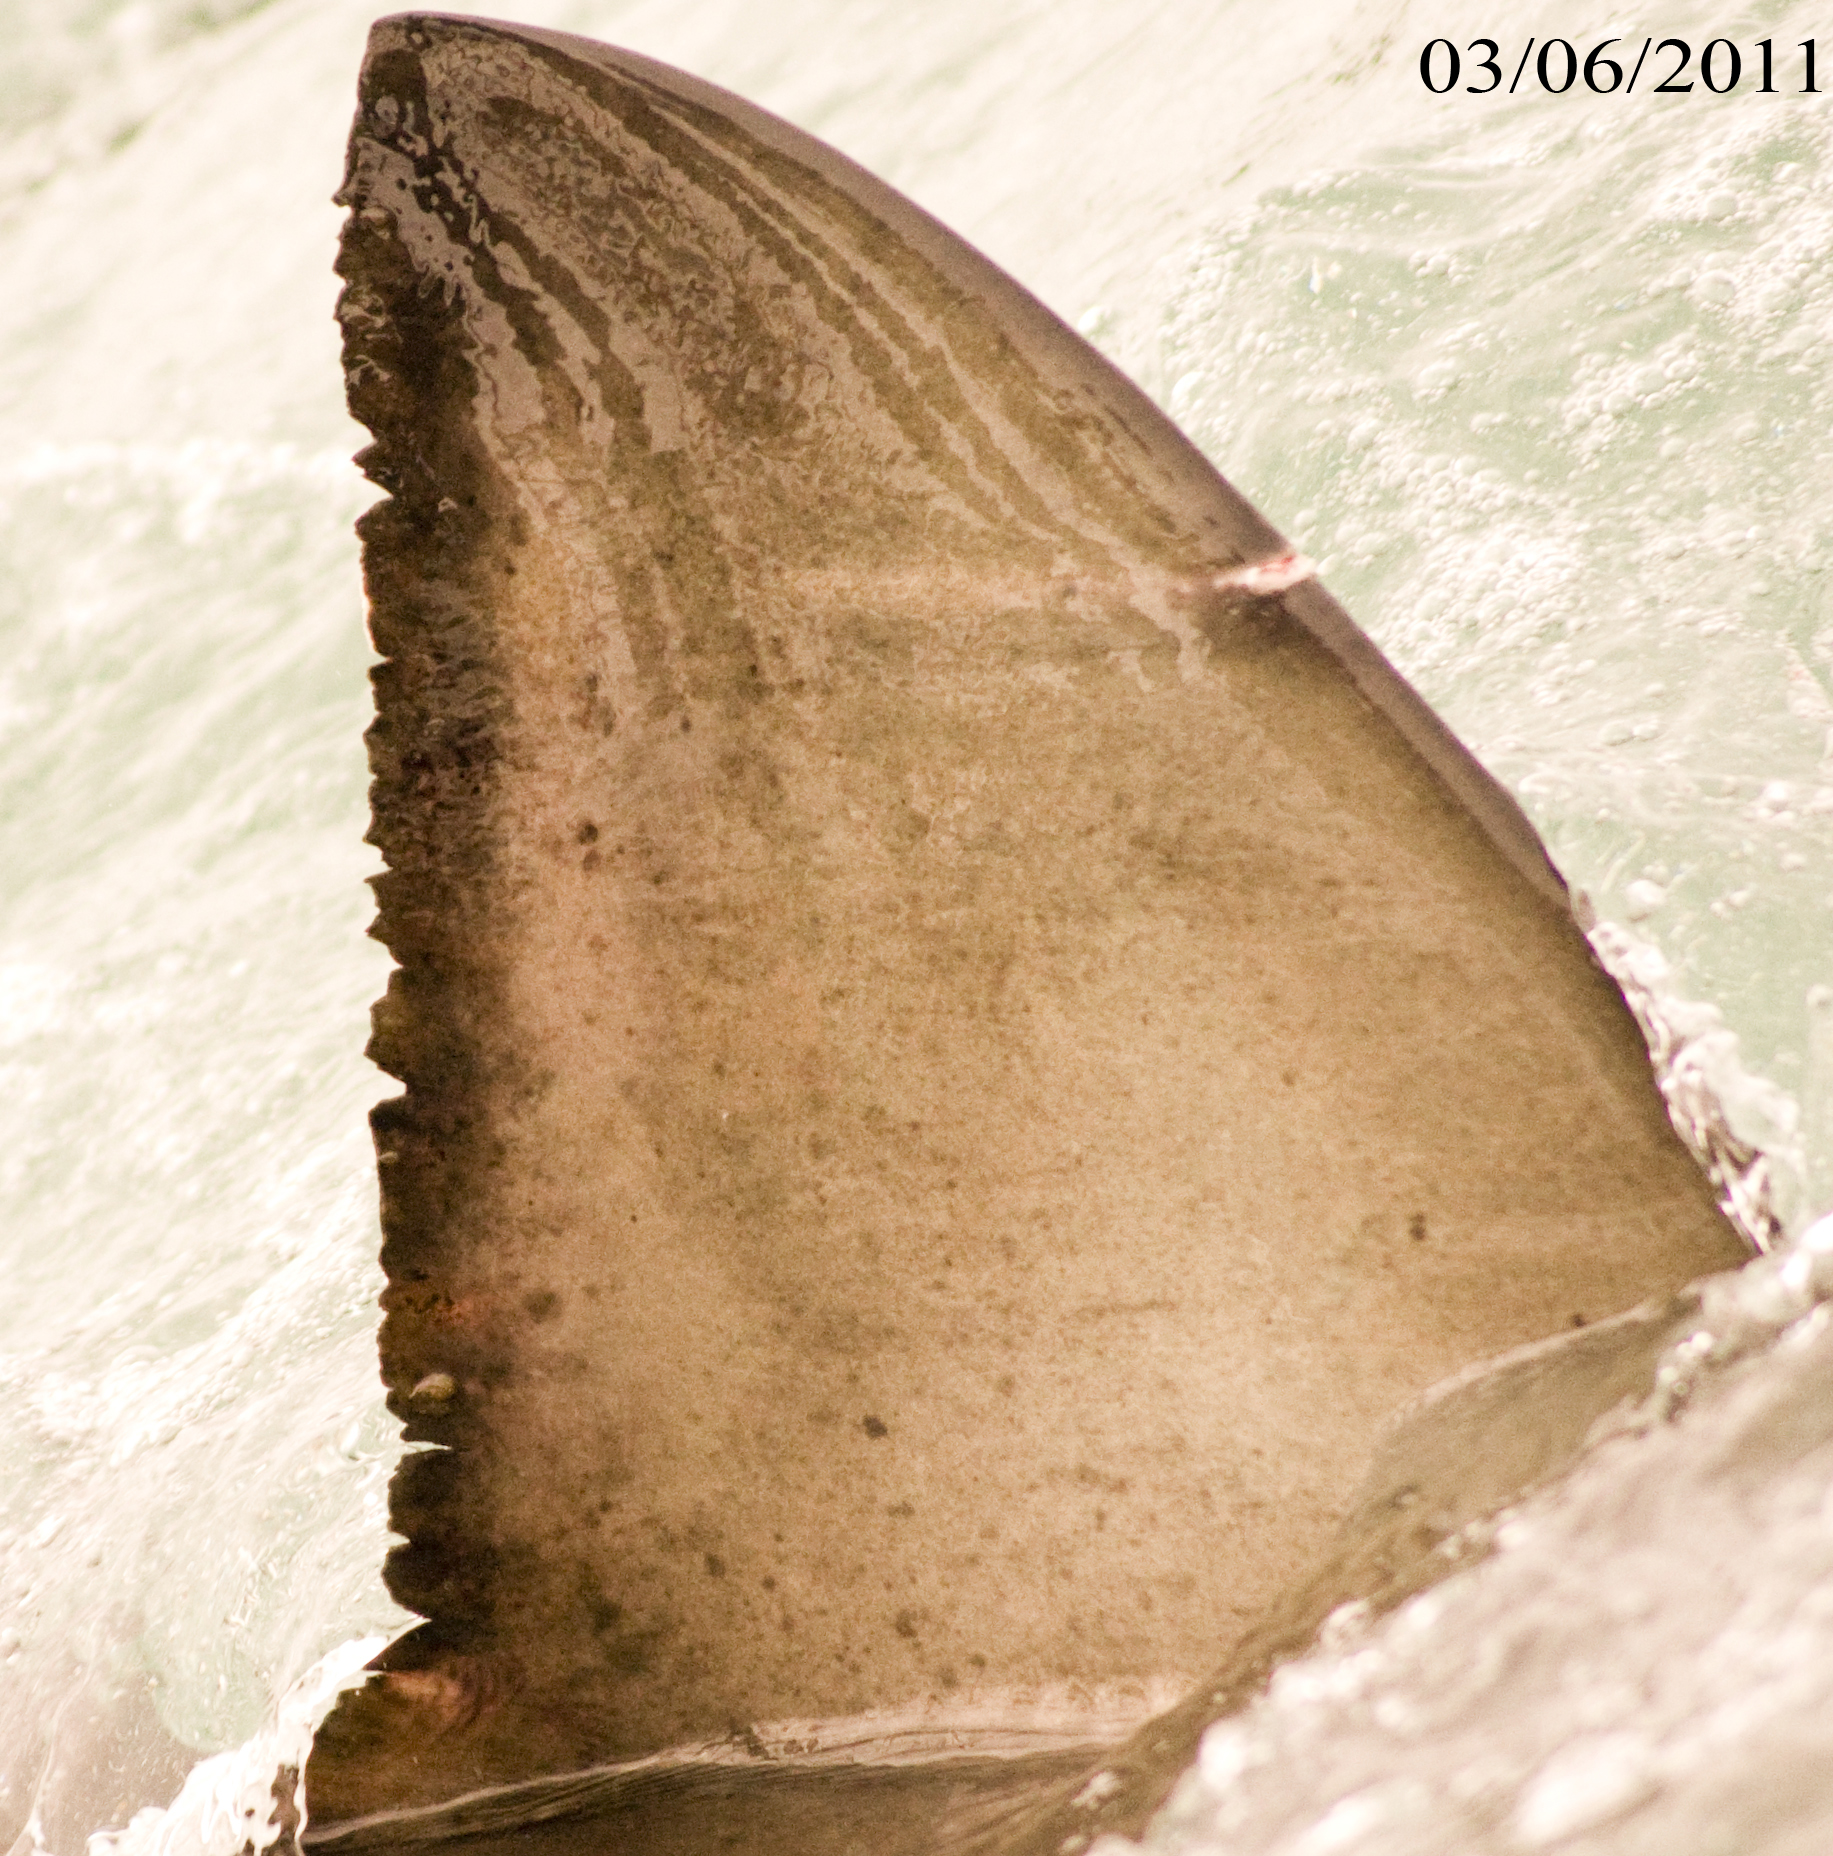
\includegraphics[width=2in]{haai3.jpg}} \quad
\subfigure[]{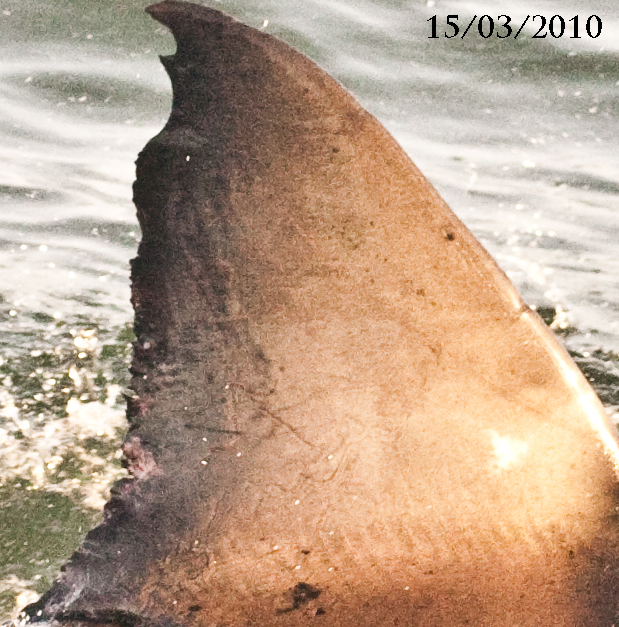
\includegraphics[width=2in]{haai5.jpg}} \quad
\subfigure[]{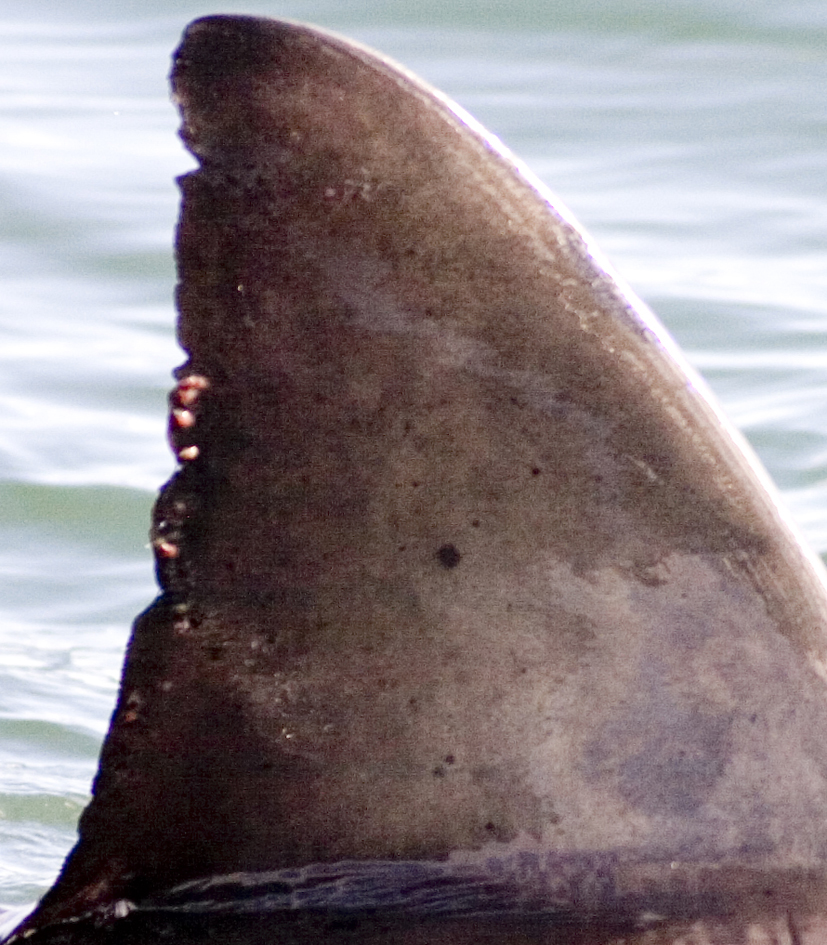
\includegraphics[width=2in]{haai6.jpg}}}
\end{figure}

\begin{figure}[H]
\centering
\mbox{\subfigure[]{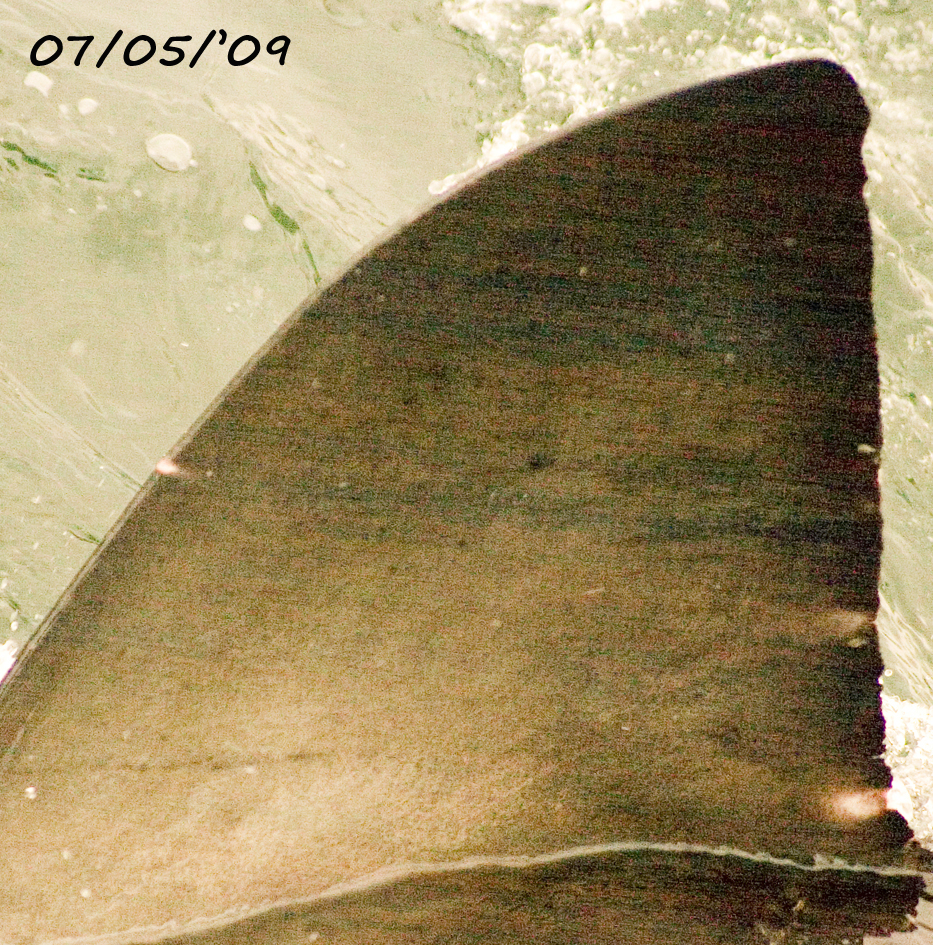
\includegraphics[width=2in]{haai7.jpg}} \quad
\subfigure[]{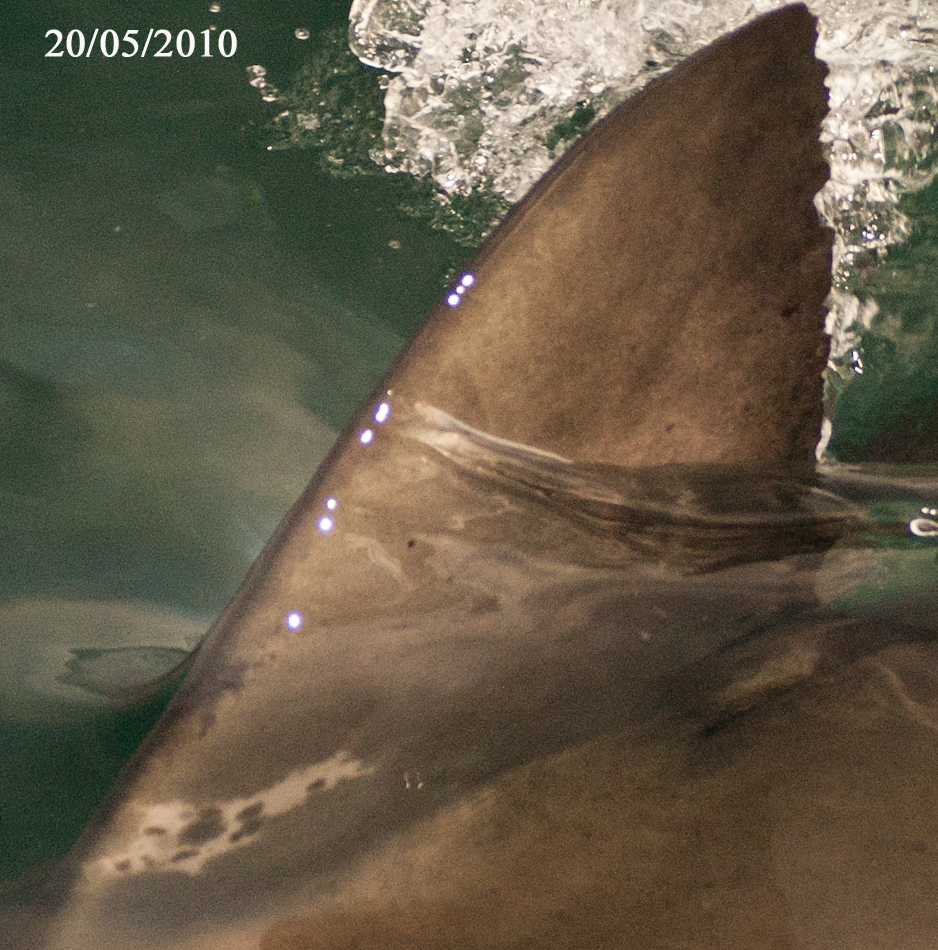
\includegraphics[width=2in]{haai8.jpg}} \quad
\subfigure[]{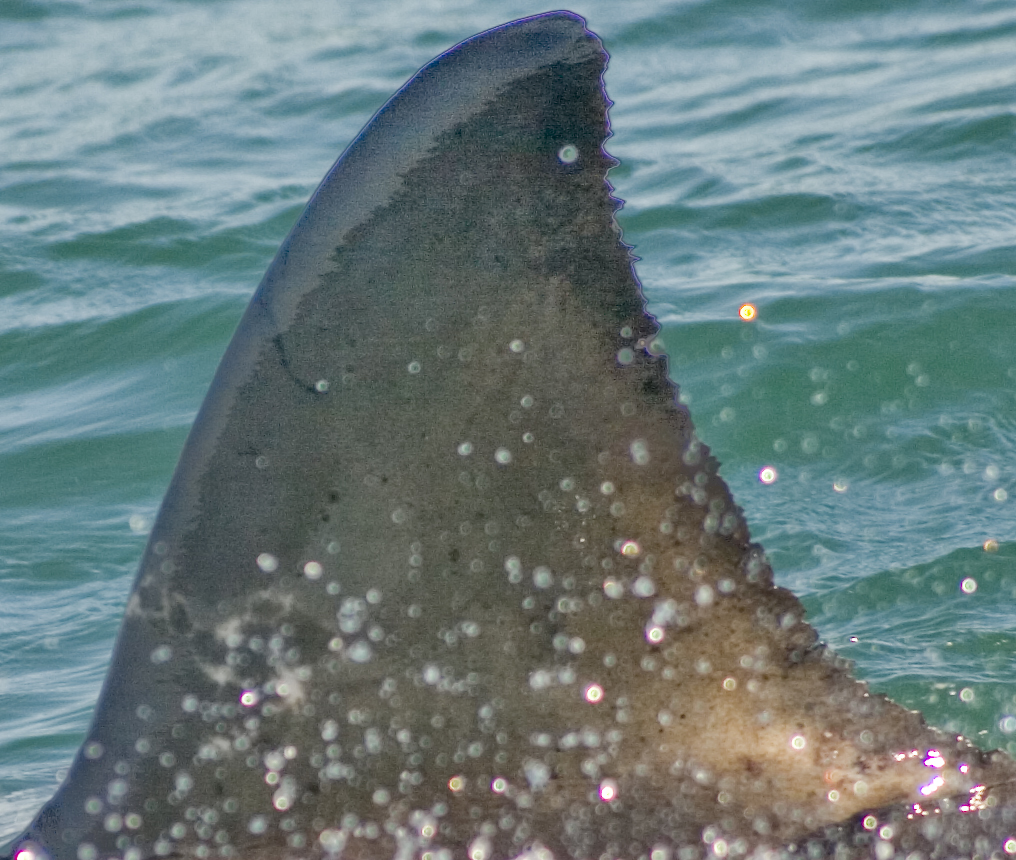
\includegraphics[width=2in]{haai9.jpg}}}
\end{figure}

\begin{figure}[H]
\centering
\mbox{\subfigure[]{\includegraphics[width=2in]{haai10.jpg}} \quad
\subfigure[]{\includegraphics[width=2in]{haai11.jpg}} \quad
\subfigure[]{\includegraphics[width=2in]{haai12.jpg}}}
\end{figure}

Note the unique dorsal part of the fin.  Although theses photos are of a good
quality, only including the fin, the foreground and background properties can
vary significantly.


\subsection{Background}
Image segmentation is well known in the field of image processing.  It consists
of partitioning a digital image into multiple segments for some or other reason.
 Usually to make the image easier to analyse.  In other words each pixel is
assigned a label and all the pixels with the same label share a certain
property.  Image segmentation is typically used to locate an object or
boundaries in an image.  Well known examples where image processing are used is
in medical imaging to locate tumours, for example, face and
fingerprint recognition and video surveillance.  See \ref{examples}.

\begin{figure}[H]
\centering
\mbox{\subfigure[]{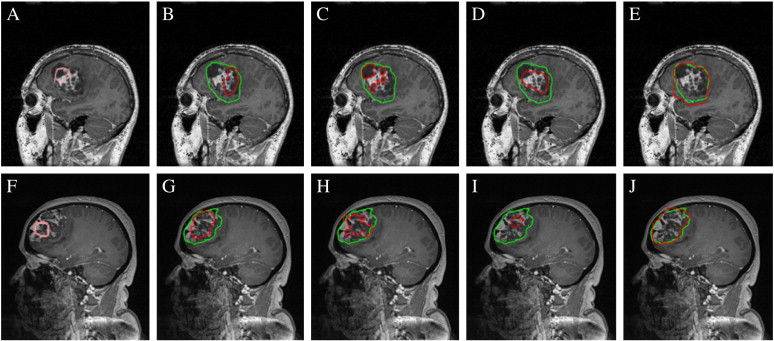
\includegraphics[width=2in]{braintumor.jpg}} \quad
\subfigure[]{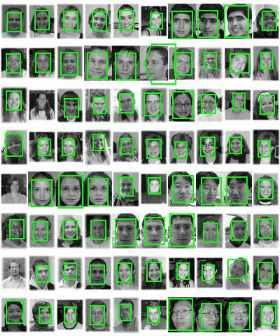
\includegraphics[width=2in]{face.jpg}}}
\caption{Image segmentation.}
\label{examples}
\end{figure}

\section{Overview of pipeline}


\subsection{Orientation}
To ease further processes, we determine the orientation of the sharkfin in the image.  The method of Principal Components Analysis (PCA) is used here.

Below we show a sampled sharkfin image where the orientation is detected using PCA.

\begin{figure}[H]
 \centering
 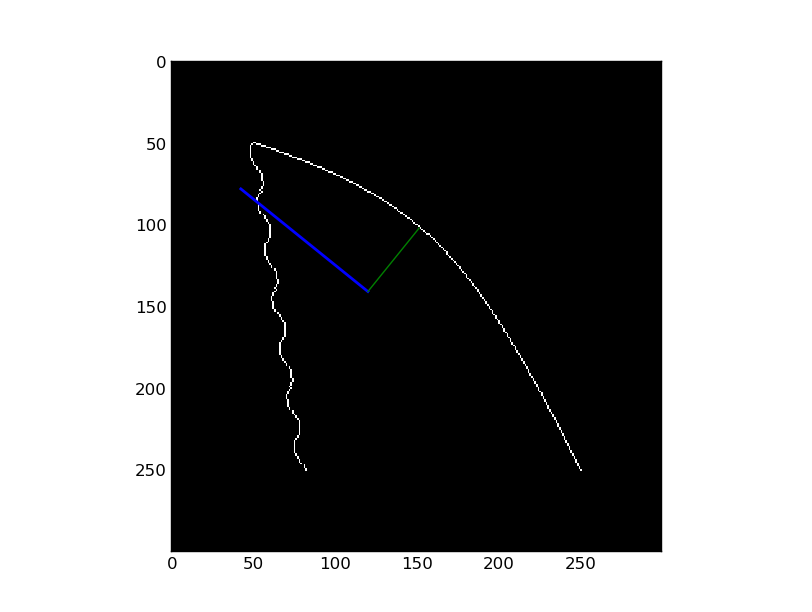
\includegraphics[width=3in]{orientation.jpg}
 \caption{Orientation detected by means of PCA.}
 \label{orientation}
\end{figure}


\subsection{Segmentation}


\subsection{Fin detection}
The objective is to identify the serrated part of dorsal sharkfin. In order to do this we need to extract the latter part of the fin such that it can be
compared with other fins.  We use the Sobel operator, well-known in edge detection, to identify the edge and ease further analysis.  
The sobel operator is a discrete differential operator that approximates the gradient of the image intensity function.
It uses two different $3 \times 3$ masks which are convolved with the original image to approximate the derivatives, both in the horizontal $x$-
and the vertical $y$-direction.  

\begin{mydef}
Convolution is defined as .
\end{mydef}

Define $A$ as the input image and $G_x$ and $G_y$ as the gradient images in the $x$-and $y$-direction respectively,
after convolving with $A$.  $M_x$ and $M_y$ is given by

\[
 M_x = \begin{pmatrix*}
        1 & 0 & -1 \\
        2 & 0 & -2 \\
        1 & 0 & -1
       \end{pmatrix*}
\mbox{ , }
 M_y = \begin{pmatrix*}
        1 & 2 & 1 \\
        0 & 0 & 0 \\
        -1 & -2 & -1
       \end{pmatrix*}
.\]

At each point in the image, the gradient approximations can be combined to give the gradient magnitude image, calculated  as
\[
 G = \sqrt{G_x^2+G_y^2}
.\]

The sobel operator applied to one of the sharkfin images is shown in \ref{sobel}.  Note that this operator only works on a grayscale image.
We can see the edge of the fin in the $G$ image on the right clearly.

\begin{figure}[H]
 \centering
 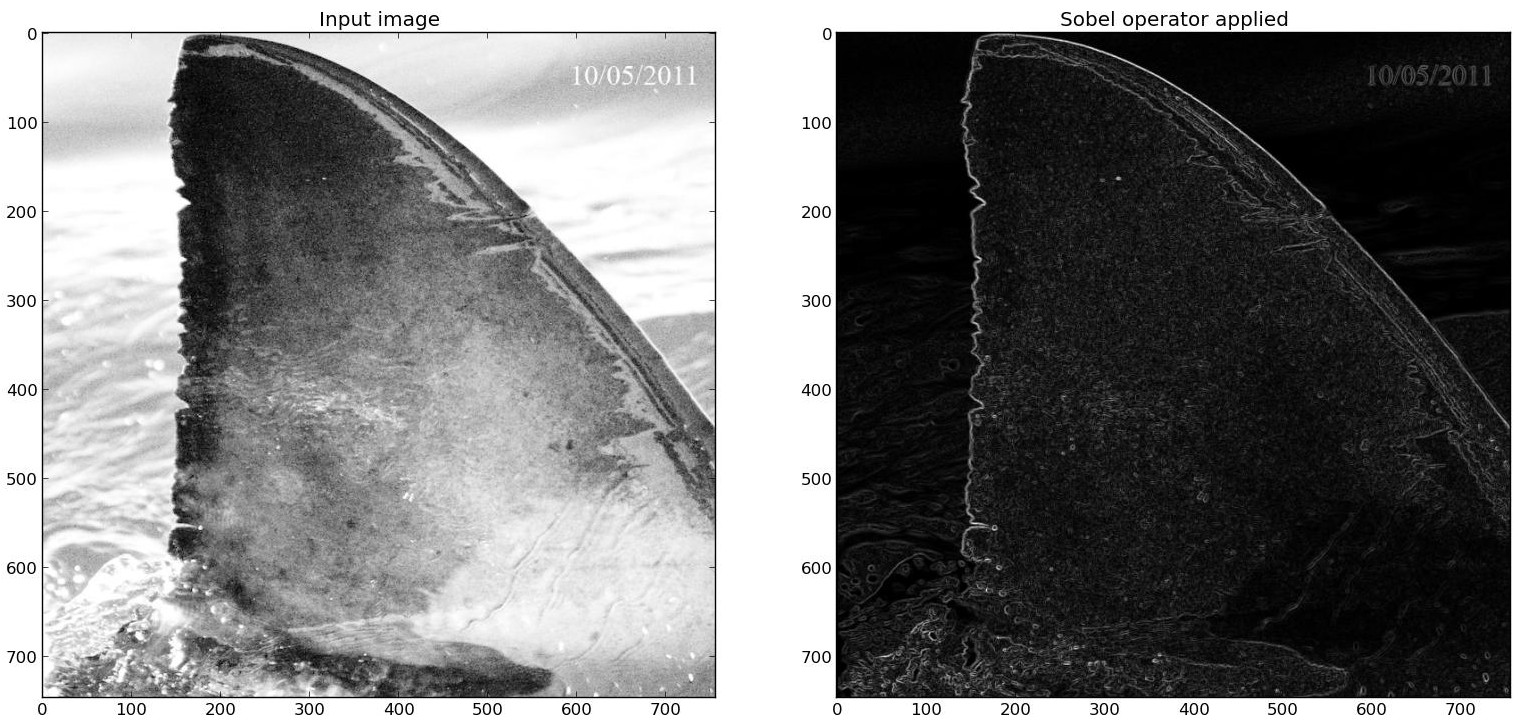
\includegraphics[width=3in]{sobel.jpg}
 \caption{The Sobel operator}
 \label{sobel}
\end{figure}

We have now managed to extract the edges from the image.

We .

\begin{figure}[H]
 \centering
 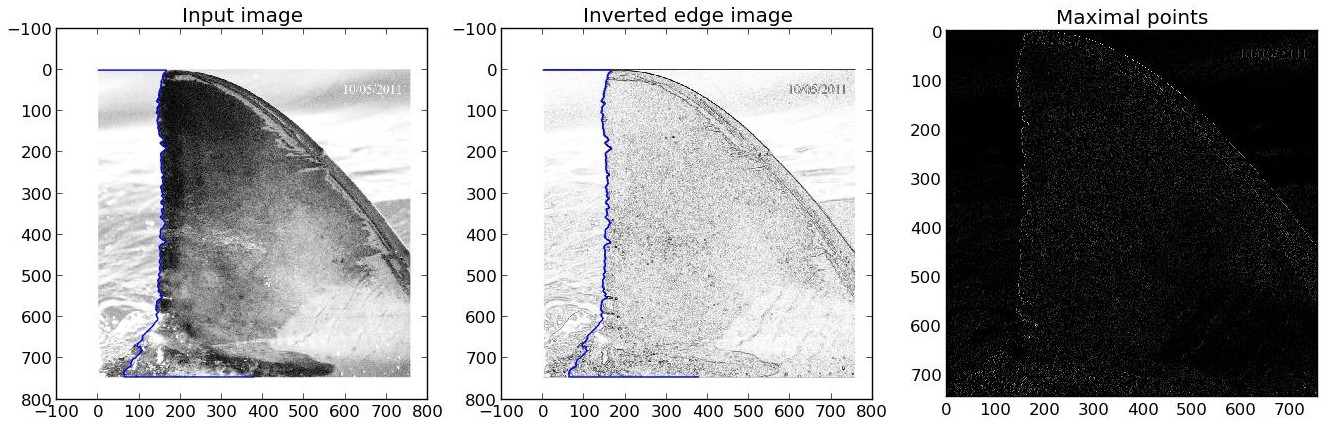
\includegraphics[width=4in]{finpath.jpg}
 \caption{Fin path detected}
 \label{fin}
\end{figure}



\subsection{Dynamic Time Warping}
Dynamic time warping (DTW) is an algorithm used for measuring the similarity between two sequences which may vary in time or speed.
It differs from normal comparison in the sense that it accomadates sequences of different lengths, warping the sequences for the best fit.
Any data that can be represented linearly can be analyzed with DTW.  For this part of the pipeline, the output from fin detection is used as input.

The path and distance is given as the output of this algorithm. The path defines the minimum cost path through the local cost matrix. 
The distance is the cost of that path. 
The lower the cost, the better the fit. For every fin compared to every other fin in the database, a cost is calculated.


\begin{figure}[H]
 \centering
 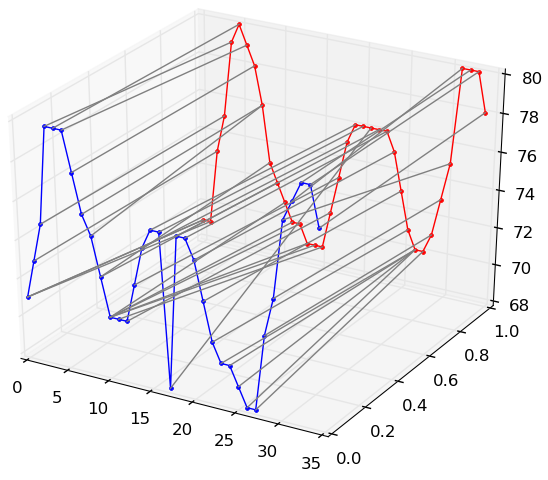
\includegraphics[width=3in]{dtw.jpg}
 \caption{Fins compared as arrays.}
 \label{dtw}
\end{figure}

\subsection{DARWIN -- Alternative software}
The DARWIN\cite{Darwin} software package is well known when it comes to aquiring important data about Great White dolphins.  It was initially implemented by undergraduate 
student Mark Allen of Eckerd College under the supervision of John Stewman.  Lately it was used to estimate the Great White
shark population in the Gansbaai area by means of shark fin identification and matching.  This claim was tested by Ms. Andreotti and she found that in only
54\% of the cases the correct matching took place, making this software highly
unreliable.  Below is an image showing the DARWIN user interface. 

\begin{figure}[H]
 \centering
 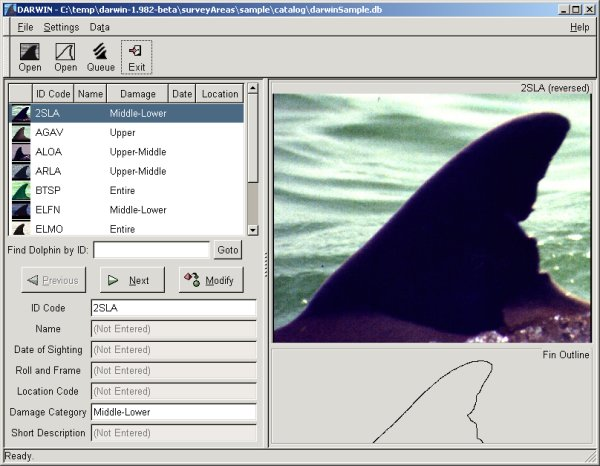
\includegraphics[width=3in]{Darwin.jpg}
 \caption{User interface}
\end{figure}

\section{Segmentation Algorithms}
\subsection{Different categories and techniques}
Segmentation algorithms can be arranged into different categories \cite{is}. 
Some of the most well-known categories are
\begin{itemize}
 \item \textbf{Thresholding}  Possibly the most basic method in the
field.  It relies on selecting the best threshold value to convert a gray-scale
image into a binary image.  Segmentation is then done on the binary image. 
 \item \textbf{Clustering} For these methods, the $K$-means algorithm
is typically used to partition an image into $K$ clusters, whereafter
segmentation will follow.
 \item \textbf{Compression-based} This method conjectures that the
optimal segmentation is the one that minimizes, when considering all possible
segmentations, the coding length of the data.
 \item \textbf{Histogram-based}  This is a very efficient method in the
sense that it only passes through all the pixels once.  Then a histogram of all
the pixels in the image is computed.  The peaks and valleys, colour intensity
can be used as a measure, are then used to locate clusters in the image.
 \item \textbf{Edge detection} Edge detection is a well-developed
field in image processing.  Region boundaries and edges are closely related,
since there are usually a sharp adjustment at region boundaries.  Edge detection
techniques can therefore be used as a bases for different segmentation
algorithms.  
 \item \textbf{Region growing} This method takes as input not only
the image, but also a set of seeds, which marks the objects to be segmented. 
Thereafter neighbouring, unallocated pixels are compared to the specific seed
point.  That is how the region grows iteratively.  The pixels are compared using
the difference between intensity value and the region's mean.  Pixels are then
allocated to a specific region if that difference is a minimum.  The process
terminates if all pixels belong to a region.  
 \item \textbf{Watershed transformation} See description in .    
 \item \textbf{Graph partitioning} This method is based on modelling
the image as a weighted, undirected graph, where the nodes represent the pixels
and the weights represent the similarity between neighbouring pixels. Then the
graph is partitioned into clusters according to a specific criterion.  Each
partition is then considered an object segment in the image.       
 \item \textbf{Trainable} Also known as Neural network segmentation,
this process involves processing the small areas of an image by means of an
artificial neural network or a set of neural networks.  Thereafter, using the
categories recognised by the network, the decision-making mechanism marks the
image accordingly and segmentation is done.
\end{itemize}

\subsection{Cellular automaton}
A cellular automaton consists of a grid of cells, where each one of the cells
can be in a finite number of states, say on and off.  This must be specified
beforehand.  Around each cell, a set of cells, called the cell's neighbourhood,
is defined.  An initial state, at time t = 0, is also assigned to each cell.  A
new generation of cells is then created according to a fixed rule or
mathematical function that determines the new state of the cell, by looking at
the current state of the cell as well as that of its neighbourhood.  This rule
is then applied to all of the cells simultaneously.  In this way, the cell's
state gets updated.  Note that the rules for each cell are the same and do not
change over time.  Two of the most common neighbourhood systems used are the Von
Neumann neighbourhood and the Moore neighbourhood which are shown below. 
Probably the most well-known example of a two dimensional automaton is Conway's
Game of Life.  See \cite{gol} for further details.

\begin{figure}[H]
\centering
\mbox{\subfigure{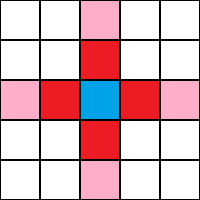
\includegraphics[width=2in]{VonNeumann.png}} \quad
\subfigure{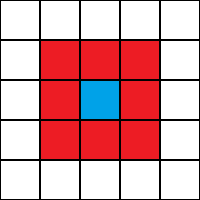
\includegraphics[width=2in]{Moore.png}}} \caption{Von Neumann and
Moore neighbourhood systems \cite{n}}
\end{figure}

\subsection{Growcut}
The Grow Cut algorithm is an interactive, multi-label segmentation algorithm for N-dimensional images.  The algorithm is based on cellular automata, i.e.,  the user labels a few pixels
and the rest of the image is then segmented automatically by a cellular automaton.  A cellular automaton consists of a grid of cells, where each one of the cells can be in 
a finite number of states, say on and off.   Around each cell, a set of cells, called the cell's neighbourhood is defined.  An initial state, at time $t = 0$, is also assigned to each cell.
A new generation of cells is then created according to a fixed rule or mathematical function that determines the new state of the cell, by looking at the current state of the cell as well
as that of its neighbourhood.  It is known that the same rules apply to each cell and do not change over time.
The algorithm is interactive, since the user can observe the segmentation and guide the algorithm in places where the segmentation is difficult to compute.
Some of the favourable properties of this algorithm is that it can do segmentation on complex images and that it works with images of any dimension. \\


\noindent The basic method on which the algorithm relies is the following.  A cellular automaton is an algorithm which is discrete in both space and time and operates on a 
lattice of pixels $p \in P \subset Z^{n}$.  A cellular automaton can be considered as a triplet, $A = (S, N, \delta)$, where $S$ is a set containing different states, $N$ is the
neighbourhood system of the cell and $\delta: S^{N} \rightarrow S $ is a transition rule.  This is the function which defines  the rule calculating the cell's state at time $t + 1$, given the states 
of the cell's neighbourhood at time $t$.  Two well known neighbourhood systems are the von Neumann and Moore neighbourhood systems.  The cell state referred to is also
considered a triplet $(l_{p}, \theta_{p}, \overrightarrow{C}_{p})$, where $l_{p}$ is the label of the cell($K$ labels in total), $\theta_{p}$ is the 'strength' of the cell and $\overrightarrow{C}_{p}$ is
the cell feature vector.  Without loss of generality it can be assumed that $\theta_{p} \in [0,1]$. 

The initial state of the pixels is set to $l_{p} = 0, \theta_{p} = 0, \overrightarrow{C}_{p} = RGB_{p}$, where $RGB_{p}$ is a three dimensional vector of the pixel's colour in 
the RGB space.  The goal of the segmentation is to assign one of the possible $K$ labels to each one of the pixels.  The user starts the segmentation by marking specific pixels as
foreground and others as background.  This sets the initial state of each pixel.  While the labels are being updated, the user can correct and guide the process if desired.  \\

\newpage
\noindent The pseudo code for the automata evolution rule is shown below. 
\begin{algorithm}[H]
\begin{algorithmic}[1]
 \State // For each cell...
 \For{$\forall p \in P$}
 \State // Copy previous state
 \State $l^{t+1}_{p} = l^{t}_{p}$;
 \State $\theta_{p}^{t+1} = \theta_{p}^{t}$;
 \State // Neighbours try to attack the current cell
 \For{$\forall q \in N(p)$}
 \If{$g(\| \overrightarrow{C}_{p} - \overrightarrow{C}_{q} \|_{2}) \cdot \theta^{t}_{q} > \theta_{p}^{t}$}
 \State $l^{t+1}_{p} = l^{t}_{q}$
 \State $\theta^{t+1}_{p} = g(\| \overrightarrow{C}_{p} - \overrightarrow{C}_{q} \|_{2}) \cdot \theta^{t}_{q}$
 \EndIf
 \EndFor
 \EndFor
\end{algorithmic}
\end{algorithm}

\noindent where $g$ is a monotonous decreasing function bounded to $[0, 1]$.  The function is given by
\[
g(x) = 1 - \frac{x}{max\| \overrightarrow{C} \|_{2}}. 
\]


\noindent The algorithm has been modified in the following way.  One of the main features that needed attention was the damping function $g$.  
By changing the exponent of the term $\frac{x}{max\| \overrightarrow{C} \|_{2}}$ to $\frac{3}{2}$, thus $\left ({\frac{x}{max\| \overrightarrow{C} \|_{2}}}\right ) ^\frac{3}{2}$,
an immediate result was seen.  The algorithm acted much more accurately around the edges.  Next, the 'defend strength' of each pixel was modified also by playing with exponents
of certain parts of the code.  A sobel filter was used in detecting the edges.  A sobel filter calculates the gradient of the intensity of each pixel, giving the direction of the largest possible increase from light to dark and also the rate of change in that specific direction.   This results in showing how abruptly or smoothly the images changes at that point and then how likely it is that that part represents an edge.  The figure below shows a sobel filter acting on a shark fin image.  The edges of the shark fin can clearly be seen.  The main purpose of these changes was to improve accuracy when detecting the edges.
\\
\begin{figure}[H]
 \centering
 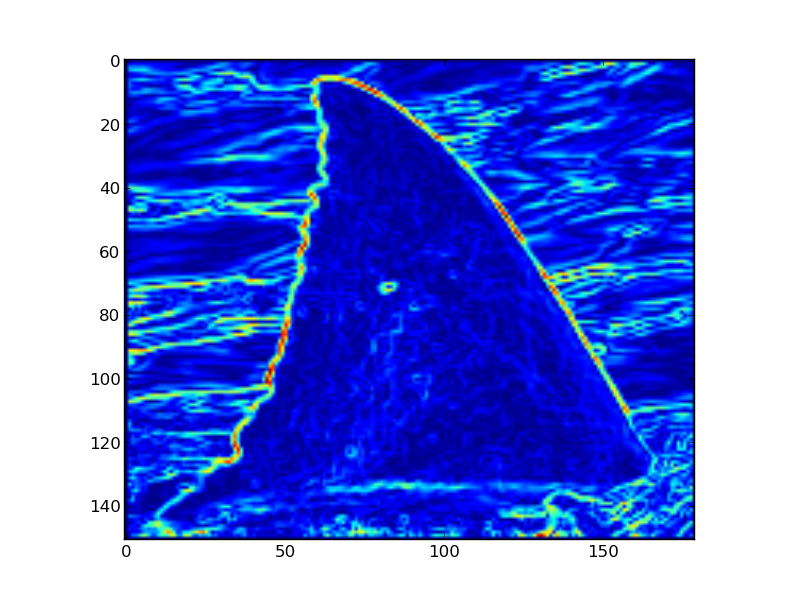
\includegraphics[width=2.5in, height=2in]{haais}
 \caption{A sobel filter applied to a shark fin image}
 \label{fin1}
\end{figure}

\newpage
\noindent Here is a comparison between the effect of the original algorithm on one of the shark fin images and the effect of the modified version of the algorithm on the same image.
\begin{figure}[H]
 \centering
 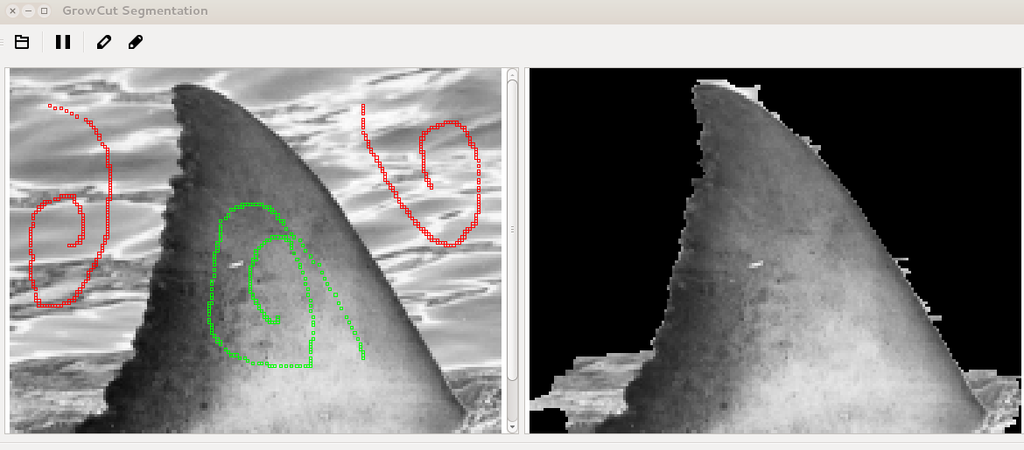
\includegraphics[width=4in, height=1.8in]{haaio}
 \caption{The effect of the original algorithm}
 \label{fin1}
\end{figure}

\begin{figure}[H]
 \centering
 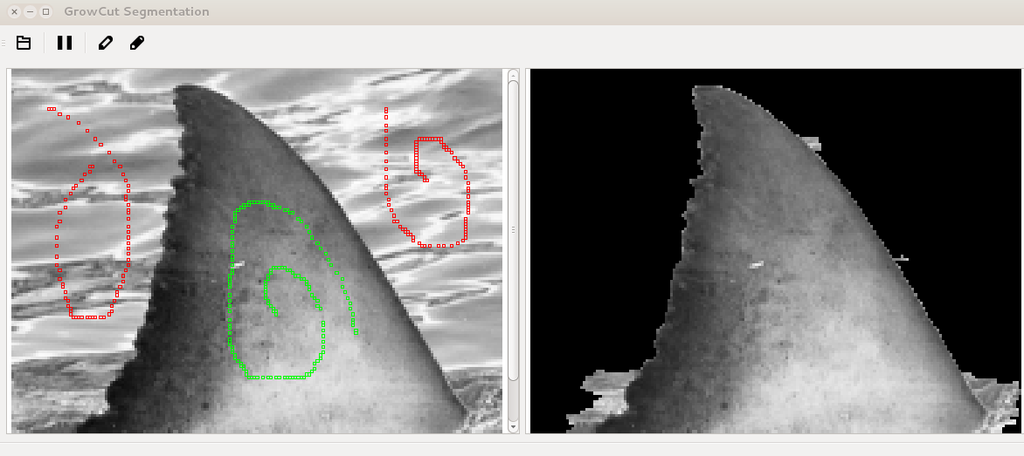
\includegraphics[width=4in, height=1.8in]{haaim}
 \caption{The effect of the modified algorithm}
 \label{fin}
\end{figure}

\noindent It can clearly be seen that the modified version gives better results around the edges, which is essential in the case of the shark fin images.  

\subsection{Random Walker}
The method, as
described in \cite{rw}, is as follows.  The user labels a few
pixels as foreground or background for example.  This is then called the seeds. 
A random walker is then released from each of the unlabelled pixels. 
Thereafter, the probability that a certain pixel's random walker first arrives
at a specific seed, is computed.  In other words, if the user labels $n$
pixels, each with a different label, then the probability that a random walker
leaving the pixel will first arrive at a certain seed, must be
computed.  The latter is done by modelling the image as a weighted graph, where
the weight of an edge reflects the similarity(intensity values) between pixels,
and then solving a system of linear equations.  The pixel is then assigned the label
of the seed for which it is most likely to reach.  The process is repeated until
each pixel is assigned a specific label. 


\subsection{Watershed}
Another segmentation algorithm is the classic watershed algorithm, as
implemented in \cite{scikit}.  The algorithm starts with user-defined markers,
called seed points, which can be viewed as little holes in the image, whereafter
pixel values are treated as a topography/landscape.  The algorithm then floods
basins from the user-defined markers until basins which attribute to different
markers meet at watershed lines.  In this case marker positions are chosen as
the local maxima of the image.  Thereafter the segmentation is done on the
gradient image.  The result of the watershed algorithm applied to a shark fin
image is shown below.

\begin{figure}[H]
\centering
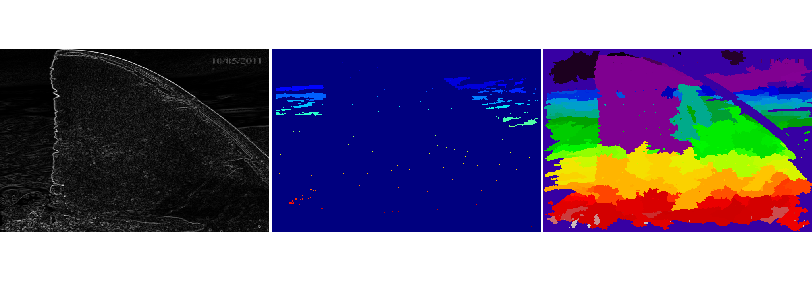
\includegraphics[width=5in,height=2in]{watershed.png} 
\label{fig1}
\caption{The watershed algorithm}
\end{figure}

\noindent The first image shows the gradient image of the original shark fin
image.  The second image shows the pixels that are identified as a local maxima.
 The third image shows how the basins flooded until watershed lines are reached.
 Putting the correct segments together, which will require a lot of hard work,
an effective segmentation can be done.

\subsection{Graphcuts}



\section{Results}
\subsection{}


\subsection{}


\subsection{}



\section{Conclusions}
\subsection{Research}


\subsection{}


\subsection{Future work}
User interface.


\newpage
\bibliography{final}

\end{document}